\documentclass[handout]{beamer}

\usepackage[utf8]{inputenc} % Language and font encoding
\usepackage[icelandic]{babel}
\usepackage[T1]{fontenc}


\usepackage{tikz}
\usepackage[listings,theorems]{tcolorbox}
\usepackage{booktabs}
\usepackage{minted} %Minted and configuration
\usemintedstyle{default}

\renewcommand{\theFancyVerbLine}{\sffamily \arabic{FancyVerbLine}}
%%%%%%%%%%%
% More math
%%%%%%%%%%%
\newcommand{\Mod}[1]{\ \text{mod}\ #1}

%%%%%%%%%%%%%%%%%%%%%%
% Beamer configuration
%%%%%%%%%%%%%%%%%%%%%%
\setbeamertemplate{navigation symbols}{}
\usecolortheme{dove}
\setbeamercolor{frametitle}{fg=white}

\usebackgroundtemplate%
{%
\vbox to \paperheight{

\includegraphics[width=\paperwidth]{Pics/hi-slide-head-2016}

\vfill
\hspace{0.5cm}
\includegraphics[width=0.3\paperwidth]{Pics/hi-von-logo}
\vspace{0.4cm}
    }%
}

\AtBeginSection[]
{
  \begin{frame}<beamer>
    \frametitle{Yfirlit}
    \tableofcontents[currentsection]
  \end{frame}
}

\setbeamerfont{frametitle}{size=\normalsize}
\addtobeamertemplate{frametitle}{}{\vspace*{0.5cm}}

%%%%%%%%%%%%%%%%%%%%%%%%%
% tcolorbox configuration
%%%%%%%%%%%%%%%%%%%%%%%%%

% Setup from: http://tex.stackexchange.com/a/43329/21638
\tcbset{%
    noparskip,
    colback=gray!10, %background color of the box
    colframe=gray!40, %color of frame and title background
    coltext=black, %color of body text
    coltitle=black, %color of title text 
    fonttitle=\bfseries,
    alerted/.style={coltitle=red, colframe=gray!40},
    example/.style={coltitle=black, colframe=green!20, colback=green!5},
}


%%%%%%%%%%%%%%%%%%%%%%%
% Further configuration
%%%%%%%%%%%%%%%%%%%%%%%
\hypersetup{colorlinks=true,pdfauthor={Eirikur Ernir Thorsteinsson},linkcolor=blue,urlcolor=blue}
\graphicspath{{./Pics/}}

\author{Eiríkur Ernir Þorsteinsson}
\institute{Háskóli Íslands}
\date{Haust 2016}

\title{Stærðfræðimynstur í tölvunarfræði}
\subtitle{Vika 4, seinni fyrirlestur}

\begin{document}

\begin{frame}
\titlepage
\end{frame}


\section{Inngangur}

\begin{frame}{Í síðasta tíma}
\begin{itemize}
 \item Reikniflækja
 \item Tímaflækjur nokkurra reiknirita
 \item Mengin $P$ og $NP$
\end{itemize}
\end{frame}

\section{Talnafræði}

\begin{frame}{Talnafræði}
\begin{itemize}
 \item Stærðfræði heiltalna kallast talnafræði
 \item Löng og mikil saga
 \begin{itemize}
  \item Fræg forn-grísk nöfn sem koma við sögu: Evklíð, Eratosþenes
 \end{itemize}
 \item Stærðfræði prímtalna fellur undir talnafræði
\end{itemize}
\end{frame}

\section{Deiling og afgangur}

\begin{frame}{Deilanleiki}
Ýmis hugtök í talnafræði krefjast skilnings á deilanleika (e. \emph{divisibility})

\begin{tcolorbox}[title=Deilanleiki]
Séu $a$ og $b$ heiltölur, $a \neq 0$, segjum við að $a$ deili (e. \emph{divides}) $b$ ef til er heiltala $c$ svo að $b = ac$, þ.e.a.s. ef $\frac{b}{a}$ er heiltala.

Þegar $a$ deilir $b$ segjum við að $a$ sé deilir (e. \emph{divisor} eða \emph{factor}) $b$ og að $b$ sé margfeldi (e. \emph{multiple}) af $a$.

Við skrifum $a | b$ þegar $a$ deilir $b$, annars $a \nmid b$.
\end{tcolorbox}
\end{frame}

\begin{frame}{Deilanleiki - dæmi}
Er $3|7$? \pause

Nei, $7/3$ er ekki heiltala. \pause

\vspace{0.5cm}
Er $3|12$? \pause

Já, $12/3$ er heiltalan $4$.
\end{frame}

\begin{frame}{Eiginleikar deilanleika}
Heiltöludeiling hefur nokkra áhugaverða eiginleika
\begin{tcolorbox}[title=Eiginleikar deilanleika]
Séu $a$, $b$ og $c$ heiltölur, $a \neq 0$, þá gildir:
\begin{enumerate}
 \item Sé $a|b$ og $a|c$, þá $a|(b+c)$
 \item Sé $a|b$, þá $a|b\cdot c$
 \item Sé $a|b$ og $b|c$, þá $a|c$
\end{enumerate}
\end{tcolorbox}
\end{frame}

\begin{frame}{Deilingarreikniritið}
Deilingarreikniritið er ekki reiknirit, heldur setning.

\begin{tcolorbox}[title=Deilingarreikniritið]
Látum $a$ og $d$ vera heiltölur, $d > 0$. 
Þá eru til heiltölur $q$ og $r$, $0 \leq r < d$ svo að $a = dq +r$.
\end{tcolorbox}

Hér er $d$ deilir, $a$ deilistofn (e. \emph{dividend}), $q$ kvóti (e. \emph{quotient}) og $r$ afgangur (e. \emph{remainder}).
\end{frame}


\begin{frame}{Kvóti og afgangur}
Um deilinn $d$, deilistofninn $a$, kvótann $q$ og afganginn $r$ má rita:
\[
 q = a \text{ div } d
\]
og
\[
 r = a \text{ mod } d
\]
\end{frame}

\begin{frame}{Dæmi um deilingu}
Hverjir eru kvótinn og afgangurinn þegar deilistofninn er $101$ og deilirinn $11$ (101/11)? \pause

Höfum
\[
 101 = 11 \cdot 9 + 2
\]

Svo kvótinn er $101 \text{ div } 11 = 9$ og afgangurinn $101 \Mod 11 = 2$.

\end{frame}

\begin{frame}{Dæmi um deilingu}
Hverjir eru kvótinn og afgangurinn þegar deilistofninn er $-11$ og deilirinn $3$ (-11/3)? \pause

Höfum
\[
 -11 = 3 \cdot (-4) + 1
\]

Svo kvótinn er $-11 \text{ div } 3 = -4$ og afgangurinn $-11 \Mod 3 = 1$.

\vspace{0.5cm}
Athugum að þó að $-11 = 3(-3) - 2$ sé satt, þá uppfyllir jafnan ekki $0 \leq r < 3$.
\end{frame}

\begin{frame}{Varúð - forritunarmál}
\begin{itemize}
 \item Forritunarmál meðhöndla deilingarafgang á ýmsa vegu
 \begin{itemize}
  \item Stundum virki (\%)
  \item Stundum föll (\texttt{mod} eða \texttt{rem})
  \item Stundum meira en eitt fall\ldots
 \end{itemize}
 \item Neikvæðar tölur sérstaklega varhugaverðar
 \begin{itemize}
  \item Stundum er deilingarafganginum leyft að vera neikvæður
  \item Stundum er $a \Mod m$ skilgreint jafnvel þó að $m$ sé neikvætt eða 0
 \end{itemize}
\end{itemize}
\end{frame}

\section{Framsetning heiltalna}

\begin{frame}{Framsetning heiltalna}
\begin{itemize}
 \item Fólk í flestum menningarheimum notar tugakerfið til að setja fram tölur
 \begin{itemize}
  \item Líklega vegna þess að við höfum 10 fingur
  \item Hafa eiginleika sem byggjast á tölunni 10: $965 = 9\cdot10^2+6\cdot10^1+5\cdot10^0$
 \end{itemize}
 \item Tölvuútreikningar byggjast oftast á grunntölunni 2 (tvíundarkerfi)
 \begin{itemize}
  \item Einnig til áttundakerfi (e. \emph{octal}) með grunntöluna 8 og sextándakerfi (e. \emph{hexadecimal}) með grunntöluna 16
  \item Áttunda- og sextándakerfistölur eru oftast notaðar til að setja tvíundarkerfistölur fram fyrir fólk
 \end{itemize}
\end{itemize}
\end{frame}

\begin{frame}{Framsetning heiltalna}
Um framsetningu heiltalna gildir:

\begin{tcolorbox}[title=Framsetning heiltalna]
Látum $b$ vera heiltölu, $b > 1$. Þá getum við sett fram jákvæðu heiltöluna $n$ á sniðinu
\[
 n = a_kb^k + a_{k-1}b^{k-1} + \ldots + a_1b + a_0
\]
þar sem $k$ er ekki-neikvæð heiltala, $a_0, a_1, \ldots, a_k$ eru ekki-neikvæðar heiltölur minni en $b$ og $a_k \neq 0$.
\end{tcolorbox}
Talað er um framsetningu með grunntölunni $b$.
\end{frame}

\begin{frame}{Reiknirit til grunntöluskipta}
Gráðugt reiknirit má nota til að skipta um grunntölu:
\begin{center}
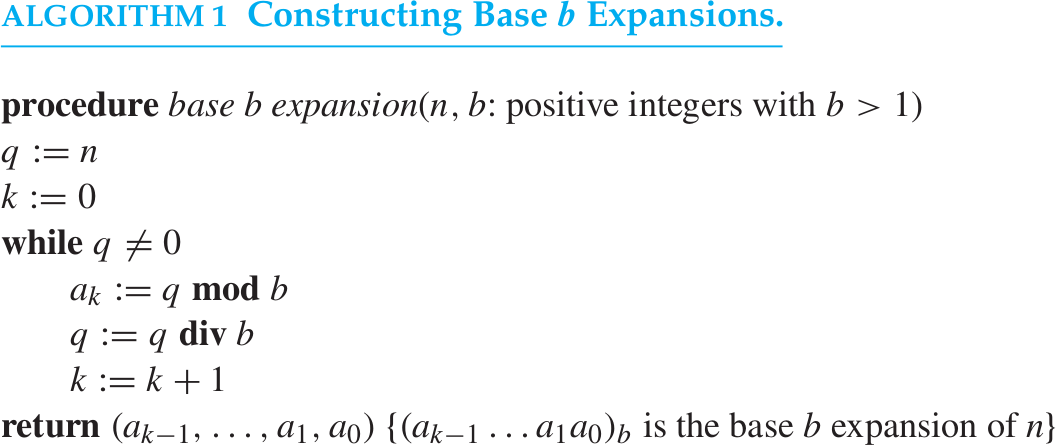
\includegraphics[width=\textwidth]{base-conversion-algorithm}
\end{center}
\end{frame}

\begin{frame}{Grunntöluskipti - dæmi}
\vspace{0.5cm}
Setjum tugakerfistöluna $(241)_{10}$ fram sem tvíundakerfistölu.
\begin{align*}
241 &= 2 \cdot 120 + 1\\
120 &= 2 \cdot 60 + 0\\
60 &= 2 \cdot 30 + 0\\
30 &= 2 \cdot 15 + 0\\
15 &= 2 \cdot 7 + 1\\
3 &= 2 \cdot 1 + 1\\
1&= 2 \cdot 0 + 1\\
\end{align*}

\vspace{-0.8cm}
Fáum afgangana $1, 0, 0, 0, 1, 1, 1, 1$ svo
\[
 (241)_{10} = (11110001)_2
\]

\end{frame}


\section{Prímtölur}

\begin{frame}{Næst}
Dulkóðun (4.6)

Seinni helmingur tímans er stoðtími.
\end{frame}


\end{document}
